\chapter{Training systems: HBM, 통신, checkpoint, publication}
\label{bg:chapter-training-systems}

Sleep-time compute를 ``남는 GPU에서 background fine-tuning''으로만 보면 실제 병목을 놓친다. Training은
weights 외에 gradients, optimizer states, activations, batches를 동시에 움직이고, 후보 artifact를
검증·복제·배포해야 끝난다. 이 장은 알고리즘을 시스템 자원으로 번역한다.

\section{한 step의 memory accounting}

Parameter 수를 $P$, element byte를 $b_w,b_g,b_o$라 하면 단순한 state lower bound는

\begin{equation}
M_{state}\approx P b_w+P b_g+kP b_o+M_{act}+M_{temp},
\end{equation}

이다. Adam의 moment가 두 개면 $k=2$이고, master weight를 별도 유지하면 한 항이 더해진다. Inference는
gradient와 optimizer state가 없지만 training은 forward activation을 backward까지 보존한다.

\concept{mixed-precision}{혼합 정밀도}는 matrix multiply와 저장 일부를 FP16/BF16/FP8로 낮추고 필요한
accumulation이나 master state는 더 높은 precision에 두어 throughput과 안정성을 trade-off한다
\parencite{micikevicius2018mixed}. ``모든 것을 16-bit''라는 뜻이 아니므로 model state별 dtype을
workbook과 checkpoint manifest에 적는다.

\concept{activation-checkpointing}{활성 체크포인팅}은 모든 intermediate activation을 저장하지 않고
일부 boundary만 보존한 뒤 backward에서 forward 일부를 재계산한다. 깊이 $n$ network의 memory를
sublinear하게 줄이는 대신 추가 compute를 쓰는 trade-off가 제시되었다
\parencite{chen2016checkpointing}. Sleep cluster에 idle FLOPs가 있어도 재계산이 wall-clock deadline과
energy budget을 넘는지 봐야 한다.

\begin{figure}[htbp]
  \centering
  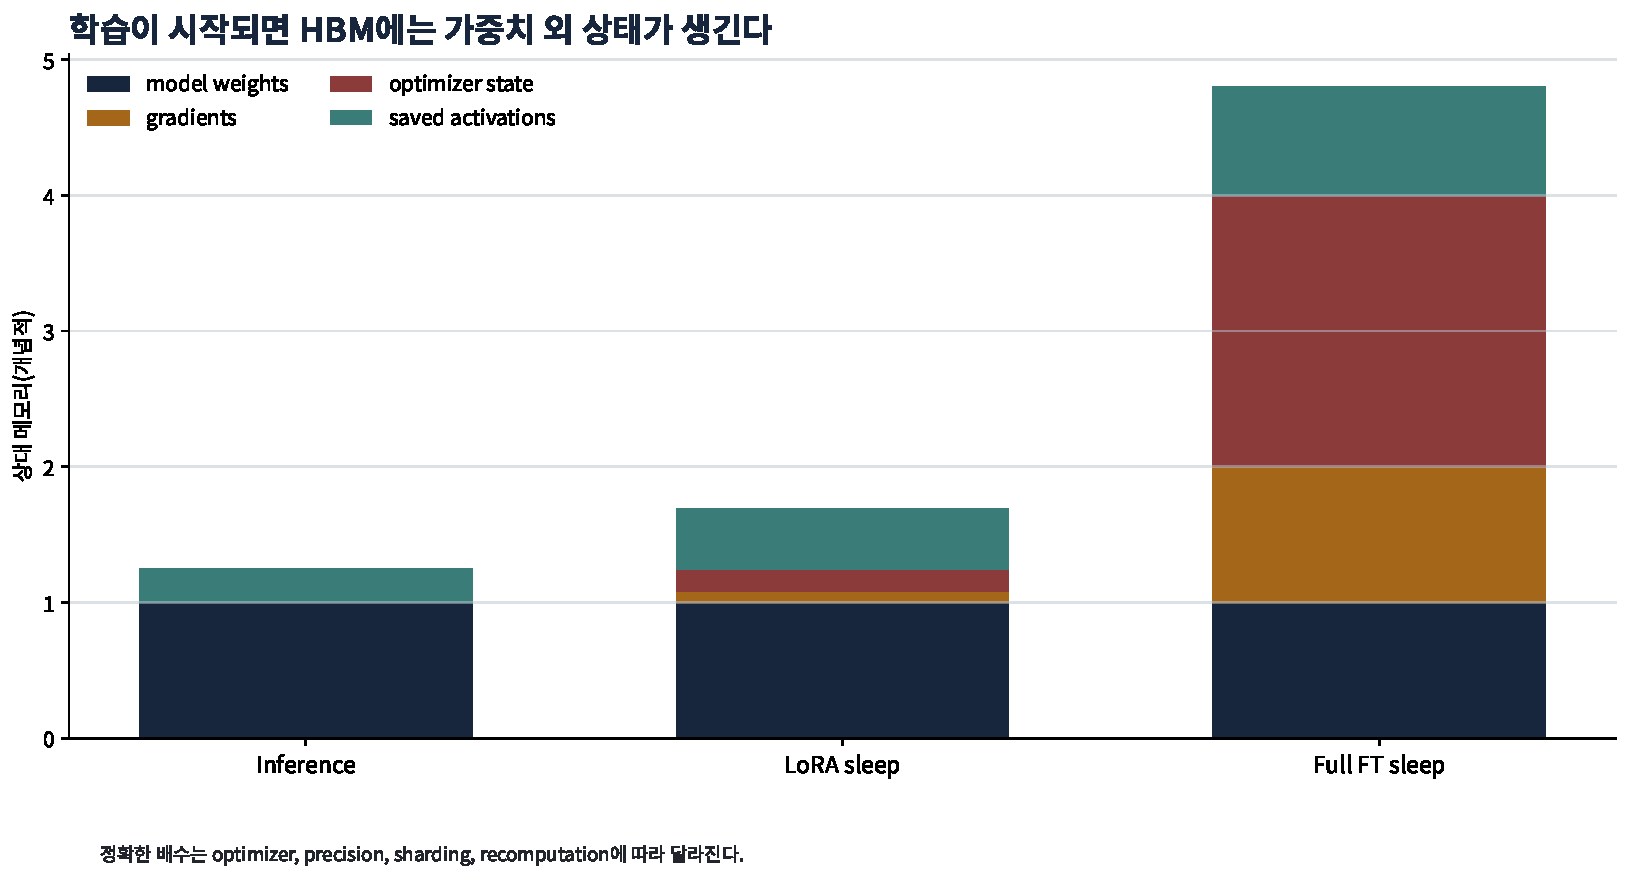
\includegraphics[width=0.94\textwidth]{figures/training-memory-cost.pdf}
  \caption{Inference, LoRA sleep, full fine-tuning sleep의 상대적 state stack. 실제 값은 optimizer,
  precision, sequence, checkpointing, sharding에 따라 달라지므로 이 그림은 구성요소 지도다.}
  \figsource{Original synthesis; SRC-STC-0030, SRC-STC-0021}{세 가지 workload마다 weights, gradients, optimizer state, activations가 층으로 쌓이며 full fine-tuning이 가장 많은 상태를 갖는 비교 그림.}
  \label{fig:bg-training-memory-cost}
\end{figure}

\section{병렬화는 무엇을 복제하고 무엇을 통신하는가}

\concept{data-parallelism}{데이터 병렬화}은 각 device에 model replica를 두고 다른 batch shard를
처리한 뒤 gradient를 all-reduce한다. Compute는 잘 확장하지만 weights와 optimizer state가 복제되고,
짧은 per-user sleep job은 batch가 작아 device utilization이 낮을 수 있다.

\concept{tensor-parallelism}{텐서 병렬화}은 한 layer의 matrix를 여러 device에 나눈다. 큰 model을
fit할 수 있지만 layer마다 collective communication이 발생한다. Megatron-LM은 transformer 내부 model
parallel pattern을 체계화했다 \parencite{shoeybi2019megatron}.

\concept{pipeline-parallelism}{파이프라인 병렬화}은 layer block을 stage로 나누고 microbatch를 흐르게
한다. GPipe는 large model training을 위한 pipeline schedule을 제시했다 \parencite{huang2019gpipe}.
Microbatch가 적으면 stage bubble이 커지므로 작은 sleep job을 개별 pipeline에 넣기보다 여러 tenant job을
privacy boundary 안에서 묶는 scheduler가 필요하다.

\concept{sharding}{샤딩}은 parameter, gradient, optimizer state를 device에 나눠 중복을 줄인다. ZeRO는
data-parallel training의 state redundancy를 단계적으로 제거한다 \parencite{rajbhandari2020zero}.
그러나 shard를 NVMe나 remote memory까지 offload하면 HBM capacity는 줄어도 step마다 read/write traffic과
tail latency가 늘 수 있다.

\begin{table}[htbp]
\centering
\caption{Sleep training job의 주요 data movement}
\label{tab:bg-training-data-movement}
\small
\begin{tabularx}{\textwidth}{p{0.19\textwidth} X X}
\toprule
경로 & 이동하는 상태 & 최적화 질문 \\
\midrule
storage $\rightarrow$ host & replay examples, provenance & sequential batch, compression, filtering locality \\
host $\rightarrow$ HBM & tokens, weights, optimizer shard & pin/prefetch, tenant isolation, reuse \\
GPU $\leftrightarrow$ GPU & activations, gradients, parameters & topology-aware collective, job packing \\
HBM $\leftrightarrow$ NVMe/CXL & cold optimizer, checkpoint, adapter & bandwidth vs recompute, endurance \\
candidate $\rightarrow$ serving & weights/delta/index/graph & atomic publish, cache warmup, rollback copy \\
\bottomrule
\end{tabularx}
\end{table}

\section{Checkpoint가 아니라 release bundle을 version한다}

\concept{versioning}{버전 관리}은 model file 이름만 바꾸는 일이 아니다. 하나의 candidate version은
base model hash, adapter/delta, optimizer continuation state, dataset manifest, code/container, random seed,
hyperparameters, evaluation report, source freeze를 묶는다. 그래야 동일 candidate를 재현하거나 어떤
source가 들어갔는지 판단할 수 있다.

\concept{rollback}{롤백}은 새 artifact pointer를 이전 검증 version으로 원자적으로 전환하고, cache와
replica를 같은 epoch으로 맞추며, 실패 candidate로 만든 후속 data를 quarantine하는 절차다. Rollback
time objective(RTO)와 최대 허용 data loss(RPO)를 external index, adapter, global weights 각각 정의한다.

\concept{publication-gate}{출판 게이트}는 candidate가 offline metric뿐 아니라 retention, privacy scope,
delete compliance, latency, resource budget을 통과할 때만 serving state로 승격하는 boundary다. Training
완료와 publication 완료를 분리하면 실패 후보를 안전하게 분석할 수 있다.

\concept{observability}{관측 가능성}은 sleep job 하나를 event ID에서 serving effect까지 trace할 수 있는
성질이다. 최소 metric은 queue wait, data bytes, H2D/D2H bytes, FLOPs, HBM peak, checkpoint bytes,
validation slices, promotion result, next-wake utility, rollback event다. 평균만이 아니라 tenant와 job size별
tail을 본다.

\section{Memory device 관점의 기회}

Sleep workload는 latency-insensitive하다고 해서 bandwidth-insensitive하지 않다. Full fine-tuning은
optimizer·gradient의 높은-capacity state, replay는 sequential/filtered reads, checkpoint는 large burst
writes, 외부 기억 compaction은 metadata-rich random I/O를 만든다. 따라서 device solution은 다음
primitive를 목표로 할 수 있다.

\begin{itemize}
  \item HBM: active weights, activation, hot optimizer shard의 bandwidth와 capacity,
  \item CXL/host memory: cold optimizer·multi-tenant adapter의 coherent tiering,
  \item NVMe: versioned checkpoint, replay log, index rebuild의 endurance와 predictable QoS,
  \item near-data processing: dedup, compression, vector/graph compaction, checksum/provenance scan,
  \item secure memory: tenant key, erase proof, immutable lineage metadata.
\end{itemize}

기회는 broad parametric sleep이 주류가 되지 않아도 남는다. External-memory consolidation, global model
refresh, checkpointing, index compaction 역시 같은 data movement와 versioning primitive를 사용하기 때문이다.

\begin{keypoint}[Roofline만으로 training job을 설명하지 못한다]
Kernel compute/HBM roofline 외에 interconnect collective, host/storage ingest, checkpoint write, validation
inference, artifact replication을 end-to-end critical path에 넣는다. Sleep window deadline을 넘기면 다음
wake 전에 publication하지 못하므로 throughput이 곧 utility다.
\end{keypoint}
